\block{Problématique}{
       { \fontsize{40}{40}\selectfont 
       
		Avec le développement des systèmes d'information et l'utilisation d'outils informatiques, il y a de plus en plus de : \vspace{0.5em}
		
		\begin{itemize}
			\item[\xmark] Fuites de données au sein des entreprises.
			\item[\xmark] Failles et problèmes de sécurité.
		\end{itemize}		        
		\vspace{0.5em}
		
		Les méthodes de sécurité classiques ne suffisent plus. Il est par conséquent primordial de mettre en place des mesures de sécurité robustes. \vspace{0.5em}
       
		Une solution à ces problèmes est d'adopter une approche biométrique. Ce type de système permet d'identifier une personne en utilisant des caractéristiques biométriques comme l'empreinte digitale, la voix, le visage ou l'iris \cite{ref_01}.       
       }
}

\block{Objectifs}{
 	{ \fontsize{40}{40}\selectfont  
	\begin{itemize}
		\item[\cmark] Développer un système d'identification basé sur une image de l'iris en passant par des techniques d'apprentissage automatique. 

		\item[\cmark] Mettre le système à disposition à travers une \textbf{API REST} destinée aux applications Web et mobiles.
	\end{itemize}
	}
}	

\block{Description du Système}{
 	{ \fontsize{40}{40}\selectfont 
 	
  	Afin de réaliser le système (Figure \ref{fig_01}) :
 	
 	\begin{itemize}
 		\item[\amark] \textbf{Scikit-Image} : \url{https://scikit-image.org/} 
 		\item[\amark] \textbf{Scikit-Learn} : \url{https://scikit-learn.org/}
 	\end{itemize}
	
	\vspace{-1.5em}
	\section{Pré-traitement}
	\vspace{-0.5em}
	Les opérations appliquées (Figure \ref{fig_02}) :
	
	\begin{itemize}
		\item[\amark] \textbf{Hough Transform} \cite{ref_02} pour détecter et extraire l'iris dans les images,
		\item[\amark] \textbf{Daugman's rubber sheet} pour transformer l'image circulaire en une rectangulaire,
	\end{itemize}		
	
	 \begin{center}
        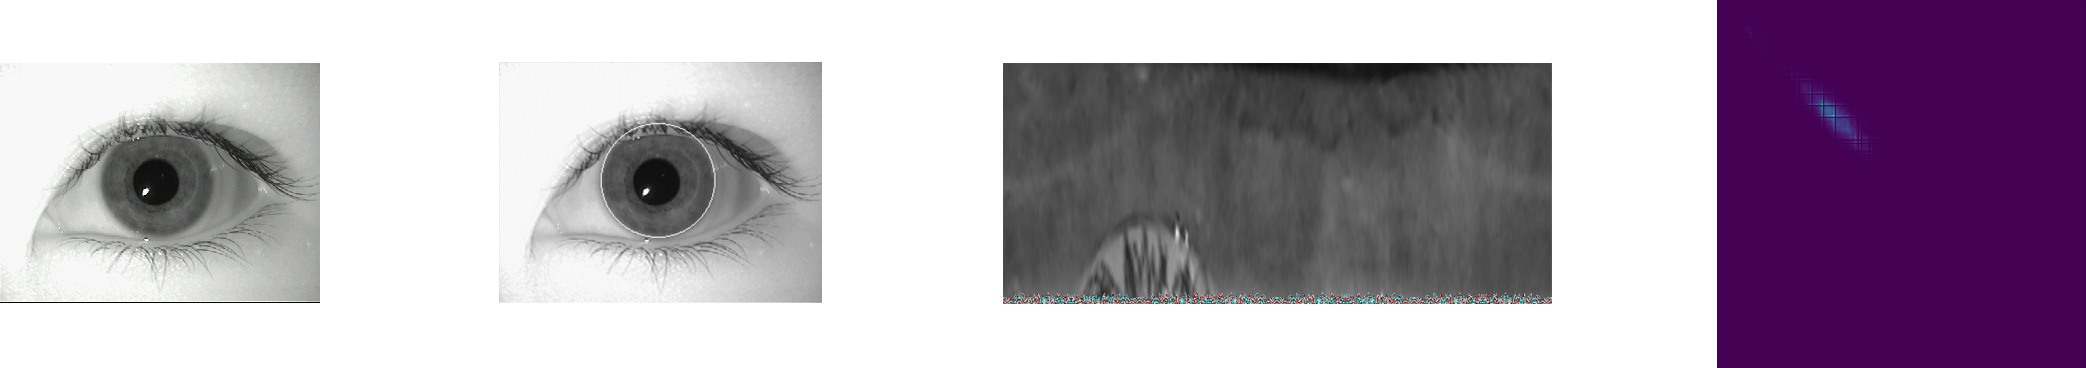
\includegraphics[width=1.0\linewidth]{processus}
        \captionof{figure}{\label{fig_02}Processus de pré-traitement (a, b et c) et aperçu de \textbf{GLCM} (d).}
    \end{center}	
    
    }
}